\documentclass[11pt,a4paper]{article}

% ----- packages -----
\usepackage[margin=2.5cm]{geometry}
\usepackage[T1]{fontenc}
\usepackage[utf8]{inputenc}
\usepackage{lmodern}
\usepackage{microtype}
\usepackage{amsmath,amssymb,amsthm,mathtools}
\usepackage{bm}
\usepackage{physics}
\usepackage{graphicx}
\usepackage{xcolor}
\usepackage{listings}
\usepackage{hyperref}
\usepackage{cleveref}
\usepackage{booktabs}
\usepackage{tikz}
\usetikzlibrary{positioning,arrows.meta,calc,shapes.geometric}

\hypersetup{
  colorlinks=true,
  linkcolor=blue!50!black,
  citecolor=blue!50!black,
  urlcolor=teal!60!black,
}

% ----- code listing style -----
\definecolor{codebg}{rgb}{0.97,0.97,0.97}
\definecolor{codekey}{rgb}{0.0,0.3,0.6}
\definecolor{codestr}{rgb}{0.55,0.10,0.10}
\definecolor{codecom}{rgb}{0.30,0.50,0.30}
\lstdefinestyle{py}{
  backgroundcolor=\color{codebg},
  basicstyle=\ttfamily\footnotesize,
  keywordstyle=\color{codekey}\bfseries,
  stringstyle=\color{codestr},
  commentstyle=\color{codecom}\itshape,
  language=Python,
  showstringspaces=false,
  breaklines=true,
  frame=single,
  framerule=0pt,
  xleftmargin=4pt,
  xrightmargin=4pt,
  tabsize=4,
}
\lstset{style=py}

% ----- shorthands -----
\newcommand{\R}{\mathbb{R}}
\newcommand{\C}{\mathbb{C}}
\newcommand{\Z}{\mathbb{Z}}
\newcommand{\E}{\mathbb{E}}
\renewcommand{\P}{\mathbb{P}}
\newcommand{\bs}{\bm{s}}
\newcommand{\btheta}{\bm{\theta}}
\newcommand{\Hop}{\hat{H}}
\newcommand{\psip}{\psi_{\btheta}}
\newcommand{\Eloc}{E_{\mathrm{loc}}}
\DeclareMathOperator{\Real}{Re}
\DeclareMathOperator{\Imag}{Im}
\DeclareMathOperator{\diag}{diag}

\theoremstyle{definition}
\newtheorem{example}{Example}
\theoremstyle{plain}
\newtheorem{proposition}{Proposition}
\newtheorem{lemma}[proposition]{Lemma}

\title{\bfseries Neural Quantum States for Lattice Spin Systems\\[2pt]
       \large A pedagogical tour of the \texttt{NQS} package}
\author{\texttt{NQS} project documentation}
\date{\today}

\begin{document}
\maketitle

\begin{abstract}
\noindent
This note explains, from first principles, every line of physics and machine
learning behind the small JAX/Flax library hosted at
\href{https://github.com/ze-bang/NQS}{\texttt{github.com/ze-bang/NQS}}.
We start from the variational principle for the quantum many-body ground
state, derive the stochastic estimator for the energy and its gradient,
develop the kernel-trick natural gradient (\textbf{MinSR}), and finally
build the three architectures shipped in the package: a translation-invariant
convolutional network (\textbf{CNN}), a fully space-group-equivariant
\textbf{GCNN}, and a Vision-Transformer ansatz (\textbf{ViT}). Each
section ends with a pointer to the file in the repository that implements it.
\end{abstract}

\tableofcontents
\bigskip

% =====================================================================
\section{The problem and the variational principle}
% =====================================================================

We are interested in the ground state of a spin-1/2 Hamiltonian on a finite
lattice with $N$ sites,
\begin{equation}
   \Hop \,:\, \mathcal{H} \to \mathcal{H}, \qquad
   \mathcal{H} = \bigotimes_{i=1}^{N} \C^{2},
\end{equation}
of dimension $D = 2^{N}$. We use the computational basis labelled by
configurations $\bs = (s_{1}, \dots, s_{N}) \in \{-1, +1\}^{N}$,
eigenstates of $\sigma^{z}_{i}$.

For $N \gtrsim 30$ the basis is too large to store, let alone diagonalise.
The \textbf{variational principle} circumvents this by parametrising the
wavefunction with a tractable function $\psip$ of the configuration:
\begin{equation}
   |\psip\rangle \;=\; \sum_{\bs} \psip(\bs)\,|\bs\rangle,
   \qquad
   \psip : \{-1,+1\}^{N} \to \C.
\end{equation}
By the Rayleigh--Ritz inequality, for any nonzero $\psip$,
\begin{equation}
\boxed{\;
   E(\btheta) \;\equiv\;
   \frac{\langle\psip|\Hop|\psip\rangle}{\langle\psip|\psip\rangle}
   \;\geq\; E_{0}.
\;}
\label{eq:variational}
\end{equation}
Minimising $E(\btheta)$ over $\btheta \in \R^{P}$ is therefore a principled
strategy. The two questions that occupy the rest of this note are:
\emph{which} $\psip$ to choose, and \emph{how} to minimise
\eqref{eq:variational} when summing $2^{N}$ configurations is impossible.

\paragraph{Scope.}
The package implements two paradigmatic models. The \emph{transverse-field
Ising model} (TFIM)
\begin{equation}
   \Hop_{\text{TFIM}}
   = -J \sum_{\langle ij \rangle} \sigma^{z}_{i}\sigma^{z}_{j}
     - h \sum_{i} \sigma^{x}_{i},
\label{eq:TFIM}
\end{equation}
and the (frustrated) Heisenberg $J_{1}$--$J_{2}$ model
\begin{equation}
   \Hop_{\text{Heis}}
   = J_{1}\!\!\sum_{\langle ij \rangle}\! \vec{S}_{i}\cdot\vec{S}_{j}
   + J_{2}\!\!\sum_{\langle\langle ij \rangle\rangle}\! \vec{S}_{i}\cdot\vec{S}_{j},
\label{eq:HeisJ1J2}
\end{equation}
both with periodic boundary conditions. Both have a sparse local
representation in the computational basis, which is what we exploit next.

\smallskip
\noindent\textit{Code:} \texttt{nqs/lattices.py}, \texttt{nqs/hamiltonians.py}.

% =====================================================================
\section{The local-energy estimator}
% =====================================================================

A direct evaluation of \eqref{eq:variational} would require the full sum
\begin{equation}
   E(\btheta)
   = \frac{\sum_{\bs,\bs'} \overline{\psip(\bs)} \,\langle\bs|\Hop|\bs'\rangle\, \psip(\bs')}
          {\sum_{\bs} |\psip(\bs)|^{2}}.
\end{equation}
The trick is to factor the numerator so that the same probability
$|\psip(\bs)|^{2}$ appears in both:
\begin{align}
   E(\btheta)
   &= \sum_{\bs} \frac{|\psip(\bs)|^{2}}{Z(\btheta)}\,
      \underbrace{\sum_{\bs'} \langle\bs|\Hop|\bs'\rangle\,
                  \frac{\psip(\bs')}{\psip(\bs)}}_{\displaystyle \Eloc(\bs)}
   \;=\; \E_{\bs \sim p_{\btheta}}\!\bigl[\Eloc(\bs)\bigr],
\label{eq:Emean}
\\[2pt]
   p_{\btheta}(\bs)
   &\;=\; \frac{|\psip(\bs)|^{2}}{Z(\btheta)},
   \qquad
   Z(\btheta) = \sum_{\bs}|\psip(\bs)|^{2}.
\end{align}
The crucial observation is that for local Hamiltonians the matrix element
$\langle\bs|\Hop|\bs'\rangle$ is non-zero only for an
$\mathcal{O}(N)$-sized set of $\bs'$ for each $\bs$. Therefore the
\textbf{local energy} $\Eloc(\bs)$ is computable in $\mathcal{O}(N)$
forward passes through the network, and an unbiased estimator of $E$ comes
from a Monte Carlo average over $N_{s}$ samples:
\begin{equation}
   \widehat{E}
   = \frac{1}{N_{s}}\sum_{k=1}^{N_{s}} \Eloc(\bs^{(k)}),
   \qquad
   \bs^{(k)} \stackrel{\text{i.i.d.}}{\sim} p_{\btheta}.
\label{eq:Ehat}
\end{equation}

\paragraph{TFIM connections.} The diagonal piece of \eqref{eq:TFIM} is
$-J \sum_{\langle ij\rangle} s_{i} s_{j}$. Each $\sigma^{x}_{i}$ flips spin
$i$, contributing one off-diagonal term per site,
\begin{equation}
   \langle \bs^{(i)} | \Hop_{\text{TFIM}} | \bs \rangle = -h,
   \qquad \bs^{(i)} = (\dots, -s_{i}, \dots).
\end{equation}
So $\Eloc(\bs)$ is a sum of one diagonal term and $N$ ratios
$\psip(\bs^{(i)})/\psip(\bs)$.

\paragraph{Heisenberg connections.} Writing $\vec S = \tfrac{1}{2}\vec\sigma$,
\begin{equation}
   \vec S_{i}\cdot \vec S_{j}
   = \tfrac{1}{4} \sigma^{z}_{i}\sigma^{z}_{j}
   + \tfrac{1}{2}\bigl(\sigma^{+}_{i}\sigma^{-}_{j} + \sigma^{-}_{i}\sigma^{+}_{j}\bigr),
\end{equation}
the off-diagonal piece swaps two opposite spins; only \emph{antiparallel}
bonds give an off-diagonal contribution. So $\Eloc(\bs)$ has at most
$|\text{bonds}|$ ratios.

\paragraph{Marshall sign.} On bipartite lattices the unfrustrated Heisenberg
model has a strictly positive ground state in a rotated basis,
$\psi(\bs) \mapsto (-1)^{N_{\uparrow,B}(\bs)}\psi(\bs)$. The package
implements this rotation by flipping the sign of every off-diagonal matrix
element, which dramatically simplifies the function the network has to
learn (no sign structure to discover when $J_{2}=0$).

\smallskip
\noindent\textit{Code:} \texttt{Hamiltonian.local\_terms()} and
\texttt{nqs.vmc.local\_energy()}.

% =====================================================================
\section{Sampling: Metropolis on the spin lattice}
% =====================================================================

We need samples from $p_{\btheta}(\bs) \propto |\psip(\bs)|^{2}$.
Direct sampling is intractable, but Metropolis--Hastings only needs
\emph{ratios}, and the network gives us
\begin{equation}
   \frac{p_{\btheta}(\bs')}{p_{\btheta}(\bs)}
   = \exp\!\bigl[2\,\Real\bigl(\log\psip(\bs') - \log\psip(\bs)\bigr)\bigr].
\end{equation}

\paragraph{Local-flip kernel.} For TFIM (which has no conservation law),
propose flipping a single random spin and accept with probability
$\min(1, p_{\btheta}(\bs')/p_{\btheta}(\bs))$.

\paragraph{Exchange kernel.} For Heisenberg in the
$S^{z}_{\text{tot}}\!=\!0$ sector, propose swapping a random
nearest-neighbour pair of opposite spins. This kernel automatically conserves
the total magnetisation, so we never leave the relevant Hilbert-space sector.

Both kernels run \texttt{n\_chains} chains in parallel inside a
single \texttt{jax.lax.scan}, with \texttt{n\_sweeps} = 2 fully
re-randomising sweeps between recorded samples.

\smallskip
\noindent\textit{Code:} \texttt{nqs/sampler.py}.

% =====================================================================
\section{Optimisation 1 — the energy gradient}
% =====================================================================

The naive route is to differentiate $\widehat{E}$ in
\eqref{eq:Ehat}. With $\log\psip(\bs)$ the natural object the network outputs,
the well-known result is\footnote{%
Derived by differentiating $E = \mathbb{E}[\Eloc]$ at fixed $\Eloc$
and noting that $\partial_i \log p = 2\,\Real \partial_i \log\psi$.
The mean subtraction term arises from the normalisation derivative.}
\begin{equation}
   \partial_{\theta_{i}} E
   = 2\,\Real\,
     \E_{p_{\btheta}}
     \bigl[(\Eloc(\bs) - \E[\Eloc])\,
           \overline{\partial_{\theta_{i}}\log\psip(\bs)}\bigr].
\label{eq:gradE}
\end{equation}
The mean subtraction is a free \textbf{control variate}: it does not change
the expectation but reduces the Monte Carlo variance, often by orders of
magnitude. Plugging \eqref{eq:gradE} into Adam already trains an NQS, but
slowly --- the next section explains why, and what to do about it.

\smallskip
\noindent\textit{Code:} \texttt{nqs.optimizer.adam\_step()}.

% =====================================================================
\section{Optimisation 2 — Stochastic Reconfiguration and MinSR}
% =====================================================================

\subsection{The Fisher--Rao geometry of \texorpdfstring{$|\psip\rangle$}{psi}}

A vanilla gradient step
$\btheta \leftarrow \btheta - \eta\,\nabla E$ is geometrically blind: it
treats the parameter space as if it were Euclidean. But two parameter
vectors that differ by a small Euclidean amount can correspond to very
different quantum states (or to the same state, in directions tangent to
re-parameterisations).

The right metric is the one inherited from the Hilbert space, the
quantum Fisher-information / Fubini--Study metric. Define the per-sample
log-derivatives
\begin{equation}
   O_{ki} \;=\; \partial_{\theta_{i}} \log\psip(\bs^{(k)}),
   \qquad k=1,\dots,N_{s},\; i=1,\dots,P,
\label{eq:O}
\end{equation}
and the (centred) covariance
\begin{equation}
   S_{ij}
   = \E_{p_{\btheta}}
     \bigl[\overline{(\partial_{i}\log\psip)}\,(\partial_{j}\log\psip)\bigr]
     - \overline{\E[\partial_{i}\log\psip]}\;\E[\partial_{j}\log\psip].
\end{equation}
\textbf{Stochastic Reconfiguration} (SR; Sorella, 1998) replaces the gradient
step by the natural-gradient step
\begin{equation}
\boxed{\;
   \btheta \;\leftarrow\; \btheta - \eta\,(S+\lambda I)^{-1}\, g,
\;}
\label{eq:SR}
\end{equation}
where $g_{i} = \partial_{\theta_{i}} E$ is the energy gradient and
$\lambda$ is a small diagonal shift (Tikhonov regulariser). Geometrically,
\eqref{eq:SR} chooses the parameter increment that, to leading order,
minimises $E(\btheta + \delta\btheta)$ subject to a fixed Fubini--Study
distance $\norm{\delta\btheta}_{S}^{2}$.

\subsection{Why \texorpdfstring{$P^{3}$}{P\textasciicircum 3} is too slow}

Build the Monte Carlo estimator directly. With centred jacobian
$\widetilde O = O - \bar O$ ($\bar O$ being the column mean) and centred
local-energy residuals $\varepsilon_{k} = \Eloc(\bs^{(k)}) - \E[\Eloc]$,
\begin{equation}
   \widehat S = \frac{1}{N_{s}}\widetilde O^{\dagger}\widetilde O \in \C^{P\times P},
   \qquad
   \widehat g = \frac{2}{N_{s}}\,\Real\bigl(\widetilde O^{\dagger}\bm{\varepsilon}\bigr).
\end{equation}
The bottleneck is the linear system $(\widehat S + \lambda I)\,\delta\btheta = \widehat g$,
of cost $\mathcal O(P^{3})$. For modern networks $P$ is $10^{5}$--$10^{7}$,
which is hopeless.

\subsection{The MinSR kernel trick (Chen \& Heyl, 2024)}

When $N_{s} \ll P$, the matrix $\widehat S = \tfrac{1}{N_{s}} \widetilde O^{\dagger}\widetilde O$
has rank at most $N_{s}$, so most of $\C^{P}$ is in its kernel. The
minimum-norm solution of the (under-determined) system
$\widetilde O\,\delta\btheta = \bm{\varepsilon}$ is exactly the SR step in
the limit $\lambda \to 0$. Solving it by the kernel trick:

\begin{proposition}[MinSR]
For real parameters and complex $\log\psip$, define the
real ``stacked'' Jacobian and residual
\begin{equation}
   \mathbf O =
   \begin{pmatrix}\Real \widetilde O \\ \Imag \widetilde O\end{pmatrix} \in \R^{2N_{s}\times P},
   \qquad
   \bm{\epsilon} =
   \begin{pmatrix}\Real\bm\varepsilon \\ \Imag\bm\varepsilon\end{pmatrix} \in \R^{2N_{s}}.
\end{equation}
The (regularised) natural-gradient direction $\delta\btheta = (\widehat S + \lambda I)^{-1} \widehat g$ equals
\begin{equation}
\boxed{\;
   \delta\btheta
   \;=\; \mathbf O^{\!\top}
         \bigl(T + \lambda I_{2N_{s}}\bigr)^{-1}
         \tfrac{1}{N_{s}}\bm{\epsilon},
   \quad
   T \,=\, \tfrac{1}{N_{s}}\,\mathbf O\,\mathbf O^{\!\top}\,\in\,\R^{2N_{s}\times 2N_{s}}.
\;}
\label{eq:minsr}
\end{equation}
\end{proposition}

\begin{proof}[Sketch]
Use the Woodbury identity / push-through identity
\begin{equation}
   (A^{\!\top}\!A + \lambda I_{P})^{-1} A^{\!\top}
   = A^{\!\top} (A A^{\!\top} + \lambda I_{2N_{s}})^{-1}
\end{equation}
with $A = \mathbf O / \sqrt{N_{s}}$. \qed
\end{proof}

The cost is now $\mathcal O(N_{s}^{2} P)$ to form $T$ and
$\mathcal O(N_{s}^{3})$ to solve --- linear in $P$. With
$N_{s} \sim 10^{3}$ and $P \sim 10^{6}$ this is several orders of magnitude
faster than the $P^{3}$ formulation, with mathematically identical results
in the limit $\lambda\to 0$.

\subsection{Computing the Jacobian \texorpdfstring{$O$}{O}}

For a network with real parameters $\btheta$ and complex output
$\log\psip = a + i\phi$, the column $O_{:,i}$ is the per-sample gradient
$\partial_{\theta_{i}}(a + i\phi)$. We compute it with two
\texttt{vmap(grad(...))} calls:
\begin{lstlisting}
real = jax.vmap(jax.grad(lambda p, x: jnp.real(log_psi_single(p, x))),
                in_axes=(None, 0))(p_flat, s)
imag = jax.vmap(jax.grad(lambda p, x: jnp.imag(log_psi_single(p, x))),
                in_axes=(None, 0))(p_flat, s)
return real + 1j * imag           # shape (N_s, P)
\end{lstlisting}

\smallskip
\noindent\textit{Code:} \texttt{nqs.vmc.minsr\_update()},
\texttt{nqs.optimizer.minsr\_step()}.

% =====================================================================
\section{The ansätze: from CNN to GCNN}
% =====================================================================

A neural quantum state is a function $\psip : \{-1,+1\}^N \to \C$. The art is
to choose a parametrisation that (i) is expressive enough to represent the
target ground state, (ii) respects the symmetries of $\Hop$, and (iii)
trains efficiently. The package ships three architectures.

\subsection{Real-/complex-valued outputs}
Each network outputs two real heads and combines them as
$\log\psip(\bs) = a(\bs) + i\,\phi(\bs)$. Working in log-space avoids
numerical underflow for unnormalised configurations and, more importantly,
makes the ratio $\psip(\bs')/\psip(\bs) = e^{\log\psip(\bs') - \log\psip(\bs)}$
that appears in $\Eloc$ trivially stable.

\subsection{The plain CNN (translation only)}
Periodic-padded convolutions are translation-equivariant: shifting the
input by one site shifts every feature map by one site. After a final
\emph{sum pooling} over the spatial dimensions and a dense readout to the
two scalar heads, the entire network is translation-\emph{invariant}:
\begin{equation}
   \log\psip(T_{\bm a}\bs) \;=\; \log\psip(\bs)
   \qquad \forall\,\bm a \in \Z_{L}\times \Z_{L}.
\end{equation}
This already captures the most important symmetry of the lattice. But it
ignores point-group symmetries (rotations by $90^\circ$ and reflections),
which the ground state of \eqref{eq:HeisJ1J2} also possesses.

\subsection{The Vision Transformer (ViT)}
Following Viteritti, Rende and Becca (PRL 2023), partition the $L\times L$
lattice into $(L/p)\times(L/p)$ patches of size $p\times p$, embed each
patch with a learned linear map plus a positional embedding, and feed the
resulting tokens through a stack of multi-head self-attention blocks. Sum
pooling over tokens yields a permutation-invariant scalar; the dense
readout then produces $a$ and $\phi$.

ViT is permutation-equivariant over patches but is not lattice-symmetric
out of the box --- the positional embeddings are learned, not enforced.
In practice it nevertheless reaches very competitive accuracies on
frustrated lattices because of its flexibility.

\subsection{Group-equivariant CNN (GCNN)}
\label{sec:gcnn}

The GCNN bakes the \emph{full space group}
\(G = T \rtimes P\) of the lattice (with $P$ the point group, here
$C_{4v}$ for the square lattice) into the architecture by construction.
Following Roth \& MacDonald (PRB 2021):

\paragraph{1.\ The group as permutations.}
For each $g \in G$, let $\pi_{g} \in S_{N}$ be its action on the $N$ sites,
$g\cdot\bs = (s_{\pi_{g}(1)}, \dots, s_{\pi_{g}(N)})$. The package builds
this representation explicitly in \texttt{nqs/groups.py} and verifies the
group axioms:
\begin{align}
   &\text{closure:}    && \mu(g, h) := g\cdot h \in G, \quad \forall g,h, \\
   &\text{identity:}   && \mu(e, g) = \mu(g, e) = g, \\
   &\text{inverse:}    && \mu(g, g^{-1}) = e, \\
   &\text{associativity:} && \mu(\mu(g,h), k) = \mu(g, \mu(h, k)).
\end{align}
The Cayley table $\mu$ and the inverse table $g \mapsto g^{-1}$ are
precomputed once and stored as integer arrays of shapes $|G|\times|G|$ and
$|G|$.

\paragraph{2.\ Lifting layer.}
The first layer ``lifts'' the input to a feature map indexed by $g$:
\begin{equation}
   f^{(0)}_{g, c}(\bs) \;=\; \sigma\!\Bigl( W_{c}\cdot (g\cdot\bs) \Bigr),
   \qquad g\in G,\; c=1,\dots,C_{0}.
\end{equation}
Concretely, for each $g$ we permute the input via $\pi_{g}$ and apply a
shared dense map $W_{c}$. The resulting tensor has shape
$(B,\,|G|,\,C_{0})$.

\paragraph{3.\ Group convolutions.}
The hidden layers act on functions $f : G \to \R^{C}$. A
\textbf{group convolution} with kernel $K : G \to \R^{C\times C'}$ is
\begin{equation}
   \bigl(K * f\bigr)_{g}
   \;=\; \sum_{h\in G} K_{g h^{-1}}\, f_{h},
   \qquad
   K_{g h^{-1}}\, f_{h} \in \R^{C'}.
\label{eq:gconv}
\end{equation}
This is the natural generalisation of a 2D convolution, replacing the
shift group $\Z^{2}$ by a general group $G$.

\begin{proposition}[Equivariance of group convolution]
For every $g_{0}\in G$, let $L_{g_{0}}$ act on functions by $(L_{g_{0}} f)_{g} = f_{g_{0}^{-1}g}$. Then
\begin{equation}
   K * (L_{g_{0}} f) \;=\; L_{g_{0}}\,(K * f).
\end{equation}
\end{proposition}
\begin{proof}
$(K * (L_{g_{0}}f))_{g} = \sum_{h} K_{gh^{-1}}\, f_{g_{0}^{-1}h}
= \sum_{h'} K_{g(g_{0}h')^{-1}}\, f_{h'}
= \sum_{h'} K_{(g_{0}^{-1}g)h'^{-1}}\, f_{h'}
= (K*f)_{g_{0}^{-1}g} = (L_{g_{0}}(K*f))_{g}.$ \qed
\end{proof}
So an arbitrary stack of group convolutions $f^{(\ell+1)} = \sigma(K^{(\ell)} * f^{(\ell)})$
preserves the action of $G$ on the feature map.

\paragraph{4.\ Implementation as gather + einsum.}
Define the \emph{shift index tensor}
\begin{equation}
   T_{g, h} \;=\; g\cdot h^{-1}, \qquad T \in \{0,\dots,|G|-1\}^{|G|\times|G|},
\end{equation}
so that \eqref{eq:gconv} becomes
\begin{equation}
   f^{(\ell+1)}_{b,g,c'}
   \;=\; \sigma\!\Bigl(
         \frac{1}{\sqrt{|G|}}\sum_{h, c} K^{(\ell)}_{T_{g,h},\, c, c'}\;
                                          f^{(\ell)}_{b, h, c}\Bigr).
\end{equation}
This is one \texttt{gather} (along the kernel's group axis) and one
\texttt{einsum} \verb|"bhc,ghcd->bgd"|. The cost is
$\mathcal O(B\,|G|^{2}\,C C')$ per layer; for $L=4,\ G = T\times C_{4v}$ we
have $|G| = 128$, which is cheap. The relevant snippet:
\begin{lstlisting}
T  = mult[:, inv]                  # (G, G)  shift table
Kg = kernel[T]                     # (G, G, C_in, C_out)
x  = jnp.einsum("bhc,ghcd->bgd", x, Kg) / jnp.sqrt(G)
\end{lstlisting}

\paragraph{5.\ Character / irrep projection.}
After $L$ group convolutions the per-sample tensor $f^{(L)} \in \R^{|G|\times C_{L}}$
transforms in the regular representation of $G$. To get a $G$-invariant
scalar, project onto the trivial irrep:
\begin{equation}
   \log\psip(\bs)
   \;=\;
   \frac{1}{|G|} \sum_{g\in G} \chi_{0}(g)\;
   \bigl[a_{\text{head}}(f^{(L)}_{g}) + i\,\phi_{\text{head}}(f^{(L)}_{g})\bigr],
\end{equation}
with $\chi_{0}(g)\equiv 1$ (the trivial character). To target a different
ground-state symmetry sector, replace $\chi_{0}$ by the character of the
appropriate one-dimensional irrep --- the rest of the architecture remains
unchanged. By orthogonality of characters this recovers the appropriate
projector $\Pi_{\text{irrep}}\,|\psip\rangle$.

\paragraph{6.\ Empirical check.}
The implementation is tested directly in code: for a randomly initialised
GCNN on the $4\times 4$ lattice with $|G| = 128$,
\begin{equation*}
\max_{g\in G,\,\bs}\,\bigl|\log\psip(g\cdot\bs) - \log\psip(\bs)\bigr| \;<\; 10^{-9}
\end{equation*}
in float32, i.e.\ at numerical precision. Symmetry is exact, not approximate.

\smallskip
\noindent\textit{Code:} \texttt{nqs/groups.py}, \texttt{nqs.ansatz.GCNN}.

% =====================================================================
\section{Putting it together: the training loop}
% =====================================================================

The whole VMC--MinSR loop is the following three-line update, repeated for
$N_{\text{steps}}$ iterations:
\begin{enumerate}
   \item \textbf{Sample.} Run the Metropolis kernel to draw $N_{s}$
         configurations from $p_{\btheta}(\bs)\propto |\psip(\bs)|^{2}$.
   \item \textbf{Local energy + Jacobian.} For each sample $\bs^{(k)}$
         compute $\Eloc(\bs^{(k)})$ and the row of $\widetilde O$ via
         \texttt{vmap(grad(...))}.
   \item \textbf{MinSR.} Solve the $2N_{s}\times 2N_{s}$ system in
         \eqref{eq:minsr} and apply the parameter update
         $\btheta \leftarrow \btheta - \eta\,\delta\btheta$.
\end{enumerate}
We additionally schedule the diagonal shift $\lambda$: starting at $10^{-2}$
and decaying multiplicatively by 0.99 every step (clipped at $10^{-4}$),
which gives strongly stabilised early dynamics and unbiased late-stage
convergence.

\smallskip
\noindent\textit{Code:} \texttt{nqs.train.train()}.

\begin{center}
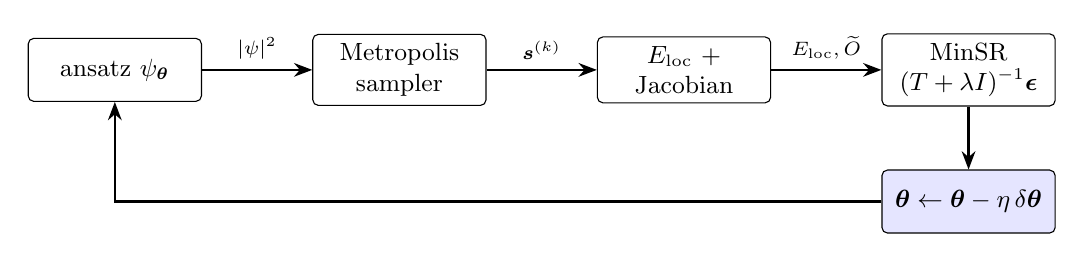
\begin{tikzpicture}[
   node distance = 14mm and 14mm,
   box/.style = {draw, rounded corners=2pt, minimum height=8mm,
                 minimum width=22mm, align=center, font=\small},
   arr/.style = {-Stealth, thick}
]
\node[box]                            (psi)   {ansatz $\psip$};
\node[box, right=of psi]              (samp)  {Metropolis\\sampler};
\node[box, right=of samp]             (eloc)  {$\Eloc$ +\\ Jacobian};
\node[box, right=of eloc]             (sr)    {MinSR\\$(T+\lambda I)^{-1}\bm\epsilon$};
\node[box, below=8mm of sr, fill=blue!10]  (upd)   {$\btheta \leftarrow \btheta - \eta\,\delta\btheta$};

\draw[arr] (psi)  -- node[above,font=\scriptsize]{$|\psi|^{2}$} (samp);
\draw[arr] (samp) -- node[above,font=\scriptsize]{$\bs^{(k)}$}  (eloc);
\draw[arr] (eloc) -- node[above,font=\scriptsize]{$\Eloc, \widetilde O$} (sr);
\draw[arr] (sr)   -- (upd);
\draw[arr] (upd) -| ($(psi.south) - (0,8mm)$) -- (psi);
\end{tikzpicture}
\end{center}

% =====================================================================
\section{Validation: comparison with exact diagonalisation}
% =====================================================================

The package includes a sparse exact-diagonalisation reference
(\texttt{nqs/ed.py}) usable up to $N \approx 22$ spins. For the provided
examples we measure the variational energy averaged over the last 20 MinSR
steps and report the relative error.

\begin{center}
\begin{tabular}{lllrrrr}
\toprule
Example & Lattice & Ansatz & \#params & \#steps
        & $E_{\text{NQS}}$ & rel.\ error\\
\midrule
\texttt{tfim\_1d.py}            & 1D, $L=8$, $h/J=1$ & CNN  & 250  & 150 & $-10.2503$ & $1.3\times10^{-4}$\\
\texttt{heisenberg\_2d.py}      & $4\times 4$        & ViT  & 6.7\,k & 120 & $-11.130$  & $8.8\times10^{-3}$\\
\texttt{heisenberg\_2d\_gcnn.py}& $4\times 4$        & GCNN & 4.7\,k & 80  & $-11.2275$ & $9.0\times10^{-5}$\\
\bottomrule
\end{tabular}
\end{center}

The GCNN reaches an accuracy roughly two orders of magnitude better than the
plain ViT, with \emph{fewer} parameters and \emph{fewer} steps. This is the
empirical payoff of building the lattice symmetries into the architecture
rather than hoping the optimiser will find them.

% =====================================================================
\section{Code map}
% =====================================================================

\begin{center}\small
\begin{tabular}{ll}
\toprule
File & Role \\
\midrule
\texttt{nqs/lattices.py}     & 1D chain, 2D square; bonds, sublattices, translations\\
\texttt{nqs/groups.py}       & space group $T \rtimes \{C_{1}, C_{4}, C_{4v}\}$, Cayley table\\
\texttt{nqs/hamiltonians.py} & TFIM and Heisenberg $J_{1}$--$J_{2}$ as sparse $\Eloc$ ops\\
\texttt{nqs/ansatz.py}       & CNN, GCNN, ViT (complex log-amplitude)\\
\texttt{nqs/sampler.py}      & Metropolis local-flip and exchange kernels\\
\texttt{nqs/vmc.py}          & local energy + Jacobian + MinSR core\\
\texttt{nqs/optimizer.py}    & MinSR step wrapper + Adam pre-trainer\\
\texttt{nqs/symmetries.py}   & post-hoc translation / $\Z_{2}$ irrep projection\\
\texttt{nqs/train.py}        & jitted training driver with diagnostics\\
\texttt{nqs/ed.py}           & sparse exact-diagonalisation reference\\
\texttt{examples/}           & runnable end-to-end scripts with ED comparison\\
\bottomrule
\end{tabular}
\end{center}

% =====================================================================
\section*{References}
% =====================================================================
\addcontentsline{toc}{section}{References}
\begin{enumerate}\itemsep=2pt
   \item G.~Carleo and M.~Troyer, \emph{Solving the quantum many-body
         problem with artificial neural networks}, Science \textbf{355},
         602 (2017).
   \item C.~Roth and A.\,H.~MacDonald, \emph{Group convolutional neural
         networks improve quantum state accuracy}, Phys.\ Rev.\ B
         \textbf{104}, 195104 (2021).
   \item C.~Roth, A.~Szabó and A.\,H.~MacDonald, \emph{High-accuracy
         variational Monte Carlo for frustrated magnets with deep neural
         networks}, Phys.\ Rev.\ B \textbf{108}, 054410 (2023).
   \item L.\,L.~Viteritti, R.~Rende and F.~Becca, \emph{Transformer
         variational wave functions for frustrated quantum spin systems},
         Phys.\ Rev.\ Lett.\ \textbf{130}, 236401 (2023).
   \item A.~Chen and M.~Heyl, \emph{Empowering deep neural quantum states
         through efficient optimization}, Nat.\ Phys.\ \textbf{20}, 1476
         (2024).
   \item S.~Sorella, \emph{Generalized Lanczos algorithm for variational
         quantum Monte Carlo}, Phys.\ Rev.\ B \textbf{64}, 024512 (2001).
   \item T.~Cohen and M.~Welling, \emph{Group equivariant convolutional
         networks}, ICML 2016.
\end{enumerate}

\end{document}
